\section{External Interface Requirements}
	\subsection{System Interfaces}
The NavUp systems’ interfaces include locating and retrieving site information (building names, addresses, etc.) based on the information retrieved from the Navigation module. The site information will be used for gathering and maintaining any information of interest with regard to the “searched” location. The acquired information about the location will be stored and pushed as a notification to the users’ interface where users can view and read it.
	\subsection{User Interfaces}
The system will allow users to find locations, so the route guidelines to the destination will be displayed on the users’ screen interface, route guidelines include a pin-point indicating users’ current positon, colored route path to the destination, and the pin-point indicating the destination. So, once the information of interest with regard to the location has been acquired, the information will be sent to the user as a notification, and the notification may be in a form of SMS, E-mail, or a push notification. The user will have an option to alter how the notifications are received, that is, either as an E-mail, push notification or an SMS.
	\subsection{Hardware Interfaces}
The Wi-Fi routers and mobile phones are the only primary hardware interfaces that may be required for the “points of interest” module. Mobile phones will be used for all the user interfaces and the functionality of the NavUp system and the Wi-Fi access points as a reference for detecting locations both indoors and outdoors.
	\subsection{Software Interfaces}
The NavUp will primarily run on mobile phones. Therefore, for compatibility requirements, the NavUp system should be hybrid, that is, it has to be compatible across most, if not all ranges of mobile smart phones and mobile operating systems, that is either Android OS, iOS, or Microsoft Windows. The system can also be web-based.
	\subsection{Communication Interfaces}
The system will frequently communicate with the campus map database, servers and the mobiles’ GPS to get locations and directions through Wi-Fi networking. Any acquired information of interest with regard to the desired location may be retrieved from the database through servers. The systems’ communication interface may also include web services.

\section{Performance Requirements}
	\subsection{Track creation/ Route update}
	The NavUp system should also keep track of the user's current location
	so to update the route displayed on the user's screen interface, however 
	the system should not necessarily update the route every after 1 second, the 
	route update can be in an interval of 7 seconds per update.
	\subsection{User login response time}
	The users will be required to login, provided that the user has
	entered correct credentials, the NavUp system should take no longer
	than 6 seconds to provide full system access to the user. However, this
	may be dependent on the internet connection bandwith.
	\subsection{Positional accuracy}
	Accuracy is one of the vital performance required for the system. The NavUp 
	system should be accurate enough to get the user’s current position, if for 
	example the user is in the building (indoor) with multiple floors, the system 
	should not necessarily determine the exact venue, but it should be in range and 
	in real time.\\\\ The system should have a good ranging accuracy. The accuracy of the 
	system is defined as the solution error, and the accuracy of the system should conform 
	to position range and the PVT (Position, Velocity and Time). This will be useful in 
	terms of “points of interest” where accuracy is very important when determining locations.
	\subsection{Proximity of notifications}
	The user will recieve any information of interest for the locations he/she visits, the amount
	of time it takes to recieve the notification shouldn't be long, this is to say, the system should 
	be responsive enough to an extent that when the user gets to the desired location, it takes no longer 
	than 25 seconds to recieve the notification.
  
	%Diagrams
	\begin{figure}[H]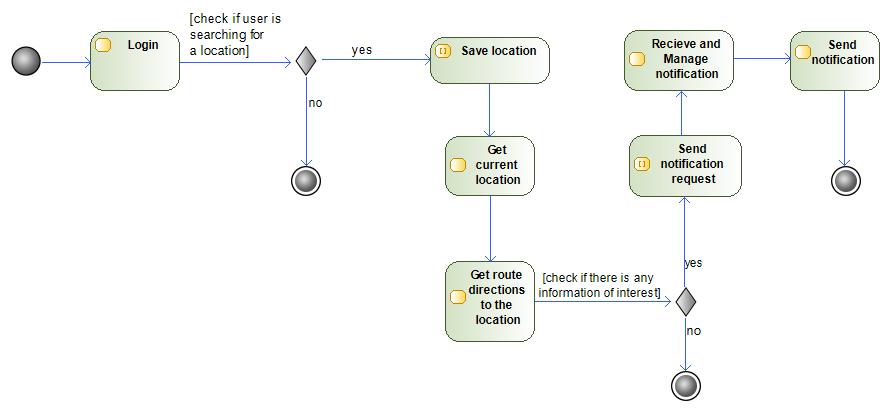
\includegraphics[width=\textwidth]{ActivityDiagram}\end{figure}
		\begin{center}Figure xx\end{center}
	\begin{figure}[H]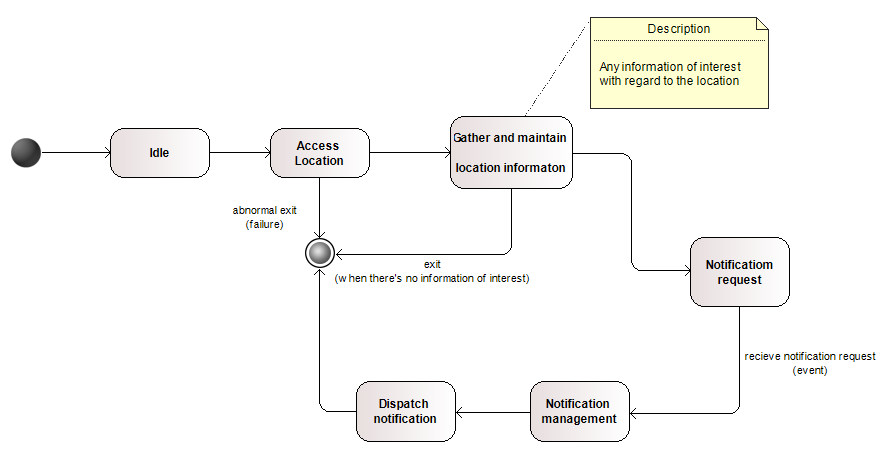
\includegraphics[width=\textwidth]{StateDiagram}\end{figure}
		\begin{center}Figure xx\end{center}
	\begin{figure}[H]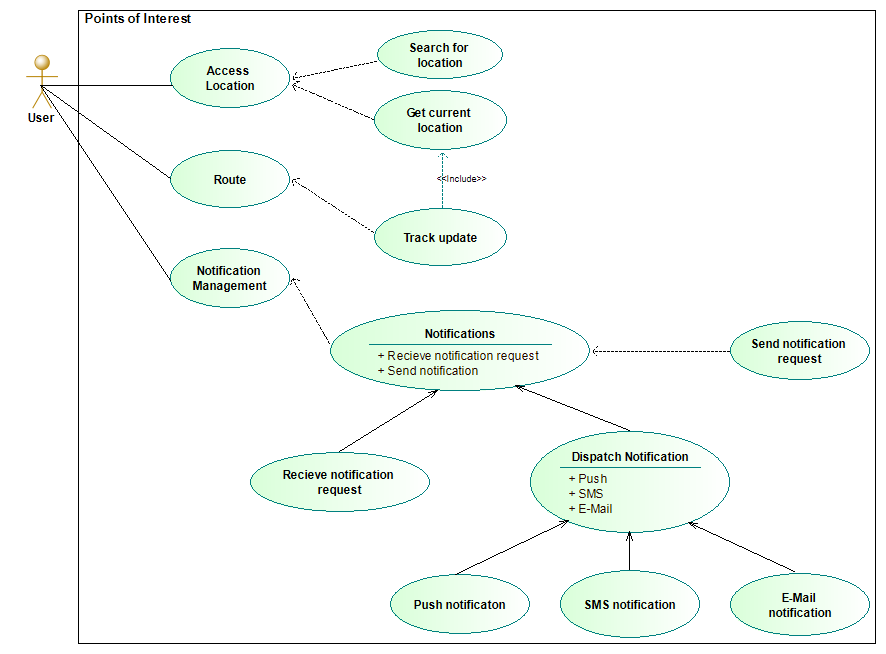
\includegraphics[width=\textwidth]{UseCaseDiagram}\end{figure}
		\begin{center}Figure xx\end{center}